\section{System Modelling}
\label{ch4:sec:system-modelling}

In this section, Section \ref{ch4:sec:system-modelling}, the underlying assumptions to validate the research are presented.
Then, the EV charging model and a BESS model are explained.
In the end of this section, the network models that are used to simulate the power distribution networks are presented.

\subsection{Assumptions}
\label{ch4:subsec:assumptions}

For this work, several underlying assumption were made to obtain the models:

\begin{enumerate}
\item
The uptake of EVs is assumed to increase and, hence, to have a significant impact on the normal operation of the low voltage distribution network.
This assumption is based on a well-established prediction that the majority of EV charging will take place at home \cite{Munkhammar2015a}.
\item
The transition from internal combustion engine-powered vehicles to EVs is assumed to not impact the users' driving behaviour.
Similar to \cite{Dallinger2012}, this assumption allows the utilisation of recent vehicle mobility data \cite{MiD2008} to generate leaving, driving and arriving probabilities, from which the EV charging demand can be determined.
\item
The transition to low carbon technologies will increase the variability of electricity demand, and therefore, grid-supporting devices, such as BESS, are anticipated to play a more important role \cite{FES2015}.
Hence, alongside a high uptake of EVs, an increased adoption of distributed BESS devices is assumed.
\item
It is assumed that BESS solutions, or more specifically battery energy storage solutions, start the simulations at 50\% SOC and are not 100\% efficient at storing and releasing electrical energy, as in \cite{Rowe2014a}.
Additionally, its utilisation will degrade the energy storage capability and performance over time, as shown in \cite{Laresgoiti2015}.
Therefore, the requirements for equal and fair storage usage is of high importance.
\item
It is assumed that the load profiles provided by the IEEE Power and Energy Society (PES) are sufficient as base load profiles for all simulations.
\end{enumerate}

\subsection{EV charging behaviour}
\label{ch4:subsec:ev-charging-behaviour}

\nomenclature[L]{$n_{s}(t)$}{Probability of starting a trip, where $n_{s}(t) \in [0, 1]$}
\nomenclature[L]{$w_{x}(t)$}{Trip distance probability for weekends ($w_{we}(t)$) and week-days ($w_{wd}(d)$), where $w_{x}(t) \in [0, 1]$}
\nomenclature[L]{$\hat{n}_x(t)$}{Predicted EV demand data, where $n_{r}(t) \in \mathbb{R}$}

From publicly-available car mobility data in \cite{Dallinger2012, MiD2008} an empirical model was developed to capture the underlying driving behaviour.
This data contained two parts, the probability of starting a trip, $n_{s}(t)$, and the probability of a trip being of a certain distance, $n_{d}(t)$.
Both probabilities are at a 15-min period, and $n_{s}(t)$ is approximated by three continuous normal distribution functions, where each is defined as:

\begin{equation}
\hat{n}_x(t) = \beta_x\frac{1}{\sigma_x\sqrt{2\pi}} \exp\left[-\frac{\left(^t/_{24}-\mu_x\right)^2}{2\sigma_x^2}\right] \;\text{where}\; t = [0, 24]
\label{ch4:equ:normal-distribution}
\end{equation}


From this definition, $\hat{n}_{m}(t)$ represents the probability distribution  of a vehicle leaving in the morning, $\hat{n}_{l}(t)$ represents the probability distribution of it leaving during lunch time, and $\hat{n}_{e}(t)$ represents the probability of it leaving during the evening.
To approximate the original probability of starting a trip, the difference between these three functions' aggregate and $n_s(t)$ needed to be minimised.
This minimisation is achieved by a Generalised Reduced Gradient (GRG) algorithm, which fits the three functions to the original data.
In order to represent a symmetric commuting behaviour, i.e. vehicles departing in the morning return during the evening, an equality amongst the three probabilities was defined as follows:

\begin{equation}
0 = \int_{0}^{24}\hat{n}_m(t) + \hat{n}_l(t) - \hat{n}_e(t) dt
\label{ch4:equ:normal-distribution-balance}
\end{equation}


The resulting parameters from the GRG fitting of the three distribution functions are tabulated in Table~\ref{ch4:tab:starting-a-trip-probability}.
Additionally, the resulting departure probabilities, as well as the original data, $n_s(t)$, are shown in Figure~\ref{ch4:fig:starting-a-trip-probability}.

\begin{table}\centering
	\begin{tabular}{cccc}
	\hline
	\textbf{Equation} \boldmath{$\hat{n}_x(t)$} & \boldmath{$\mu_x$} \textbf{(Mean)} & \boldmath{$\sigma_x$} \textbf{(SD)} & \boldmath{$\beta_x$} \textbf{(Weight)} \\
	\hline
	$\hat{n}_m(t)$ & 0.3049 & 0.0488 & 0.00206 \\
	$\hat{n}_l(t)$ & 0.4666 & 0.0829 & 0.00314 \\
	$\hat{n}_e(t)$ & 0.7042 & 0.0970 & 0.00521\\
	\hline
	\end{tabular}
	\caption{Parameters for normal distributions.}
	\label{ch4:tab:starting-a-trip-probability}
\end{table}


\begin{figure}\centering
	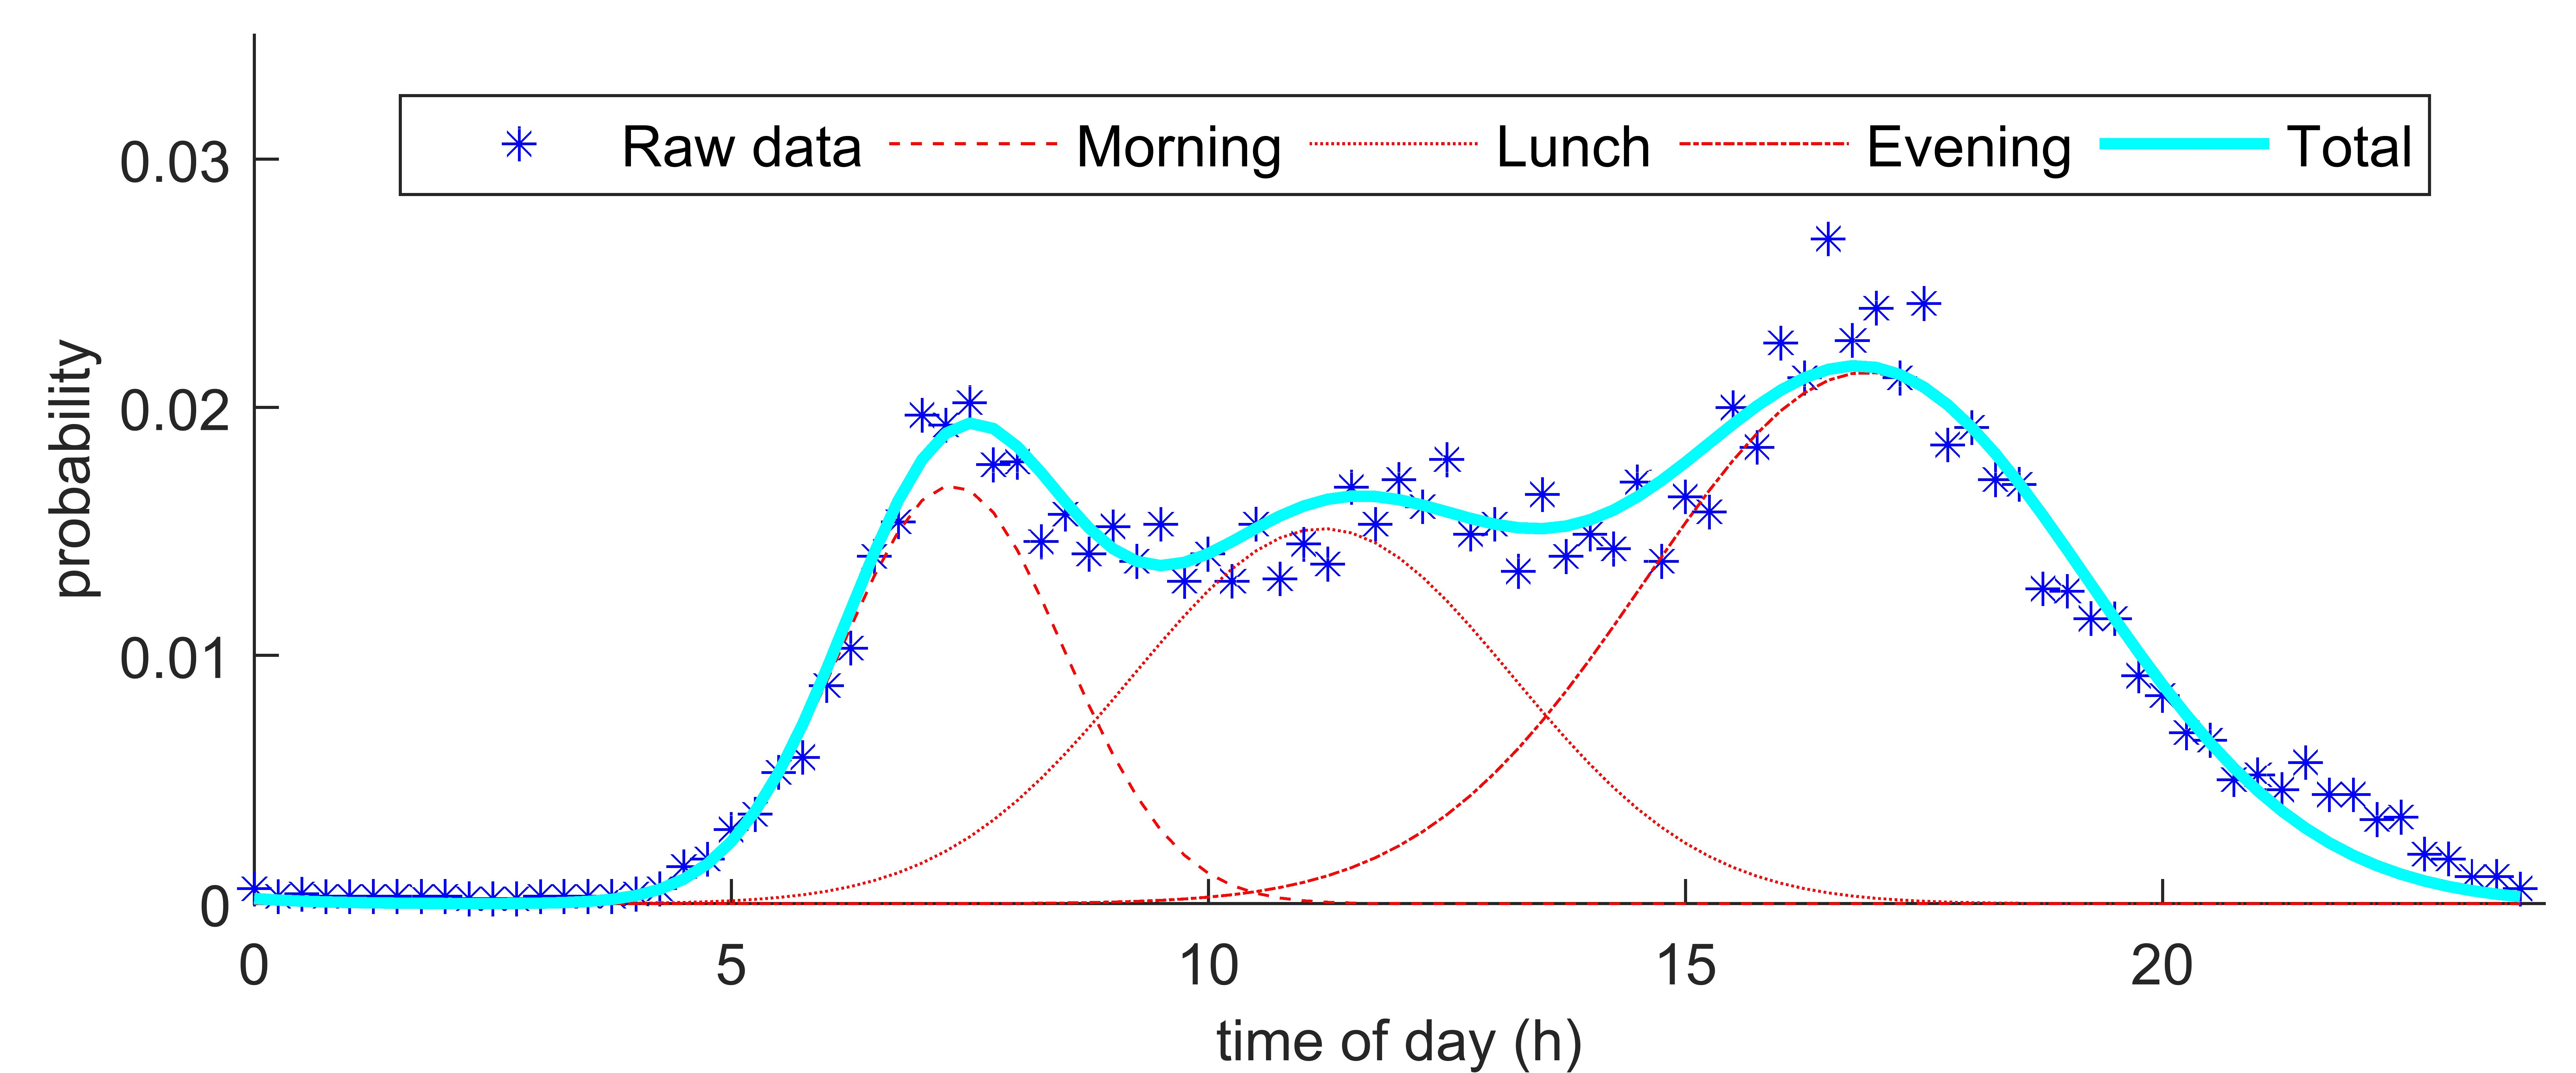
\includegraphics[width=0.8\textwidth]{_chapter4/fig/starting-a-trip-probability}
	\caption{The probability of starting a trip at a particular time during a weekday, extrapolated into three normal distributions (RMS error: $9.482\%$).}
	\label{ch4:fig:starting-a-trip-probability}
\end{figure}


The second statistical data, i.e. the data capturing the probability distribution of a trip being of a certain distance, $w_x(t)$, was also extracted from the dataset and approximated.
This was done for both the weekdays $w_{wd}(d)$ and weekends $w_{we}(d)$.
The Weibull function was chosen to be fitted against the extracted probability distributions and is defined as:

\begin{equation}
\hat{w}_x(\gamma_x,k_x,d) :=
	\begin{cases}
		\frac{k_x}{\gamma_x}\left(\frac{d}{\gamma_x}\right)^{k_x-1}\exp\left[-\left(\frac{d}{\gamma_x}\right)^{k_x}\right] &\text{if } d \geq 0 \\
		0 &\text{if } d < 0
	\end{cases}
	\label{ch4:equ:weibull-distribution}
\end{equation}


Performing the curve fitting using the GRG optimisation algorithm, a weekday trip distance distribution, $\hat{w}_{wd}(d)$, and a weekend trip distribution, $\hat{w}_{we}(d)$, could be estimated.
The computed function parameters for these two estimated distribution functions are tabulated in Table~\ref{ch4:tab:trip-distance-probailility}.
Their resulting probability distributions are plotted for comparison against the real data, $w_{wd}(d)$ and $w_{we}(d)$, in Figure~\ref{ch4:fig:trip-distance-probability}.

\begin{table}\centering 
	\begin{tabular}{ccc}
	\hline
	\textbf{Equation} \boldmath{$\hat{w}_x(d)$} & \boldmath{$\gamma_x$} \textbf{(Scale)} & \boldmath{$k_x$} \textbf{(Shape)} \\
	\hline
	$\hat{w}_{wd}(t)$ & 15.462 & 0.6182 \\
	$\hat{w}_{we}(t)$ & 38.406 & 0.4653\\
	\hline
	\end{tabular}
	\caption{Parameters for Weibull distributions.}
	\label{ch4:tab:trip-distance-probailility}
\end{table}


\begin{figure}\centering
	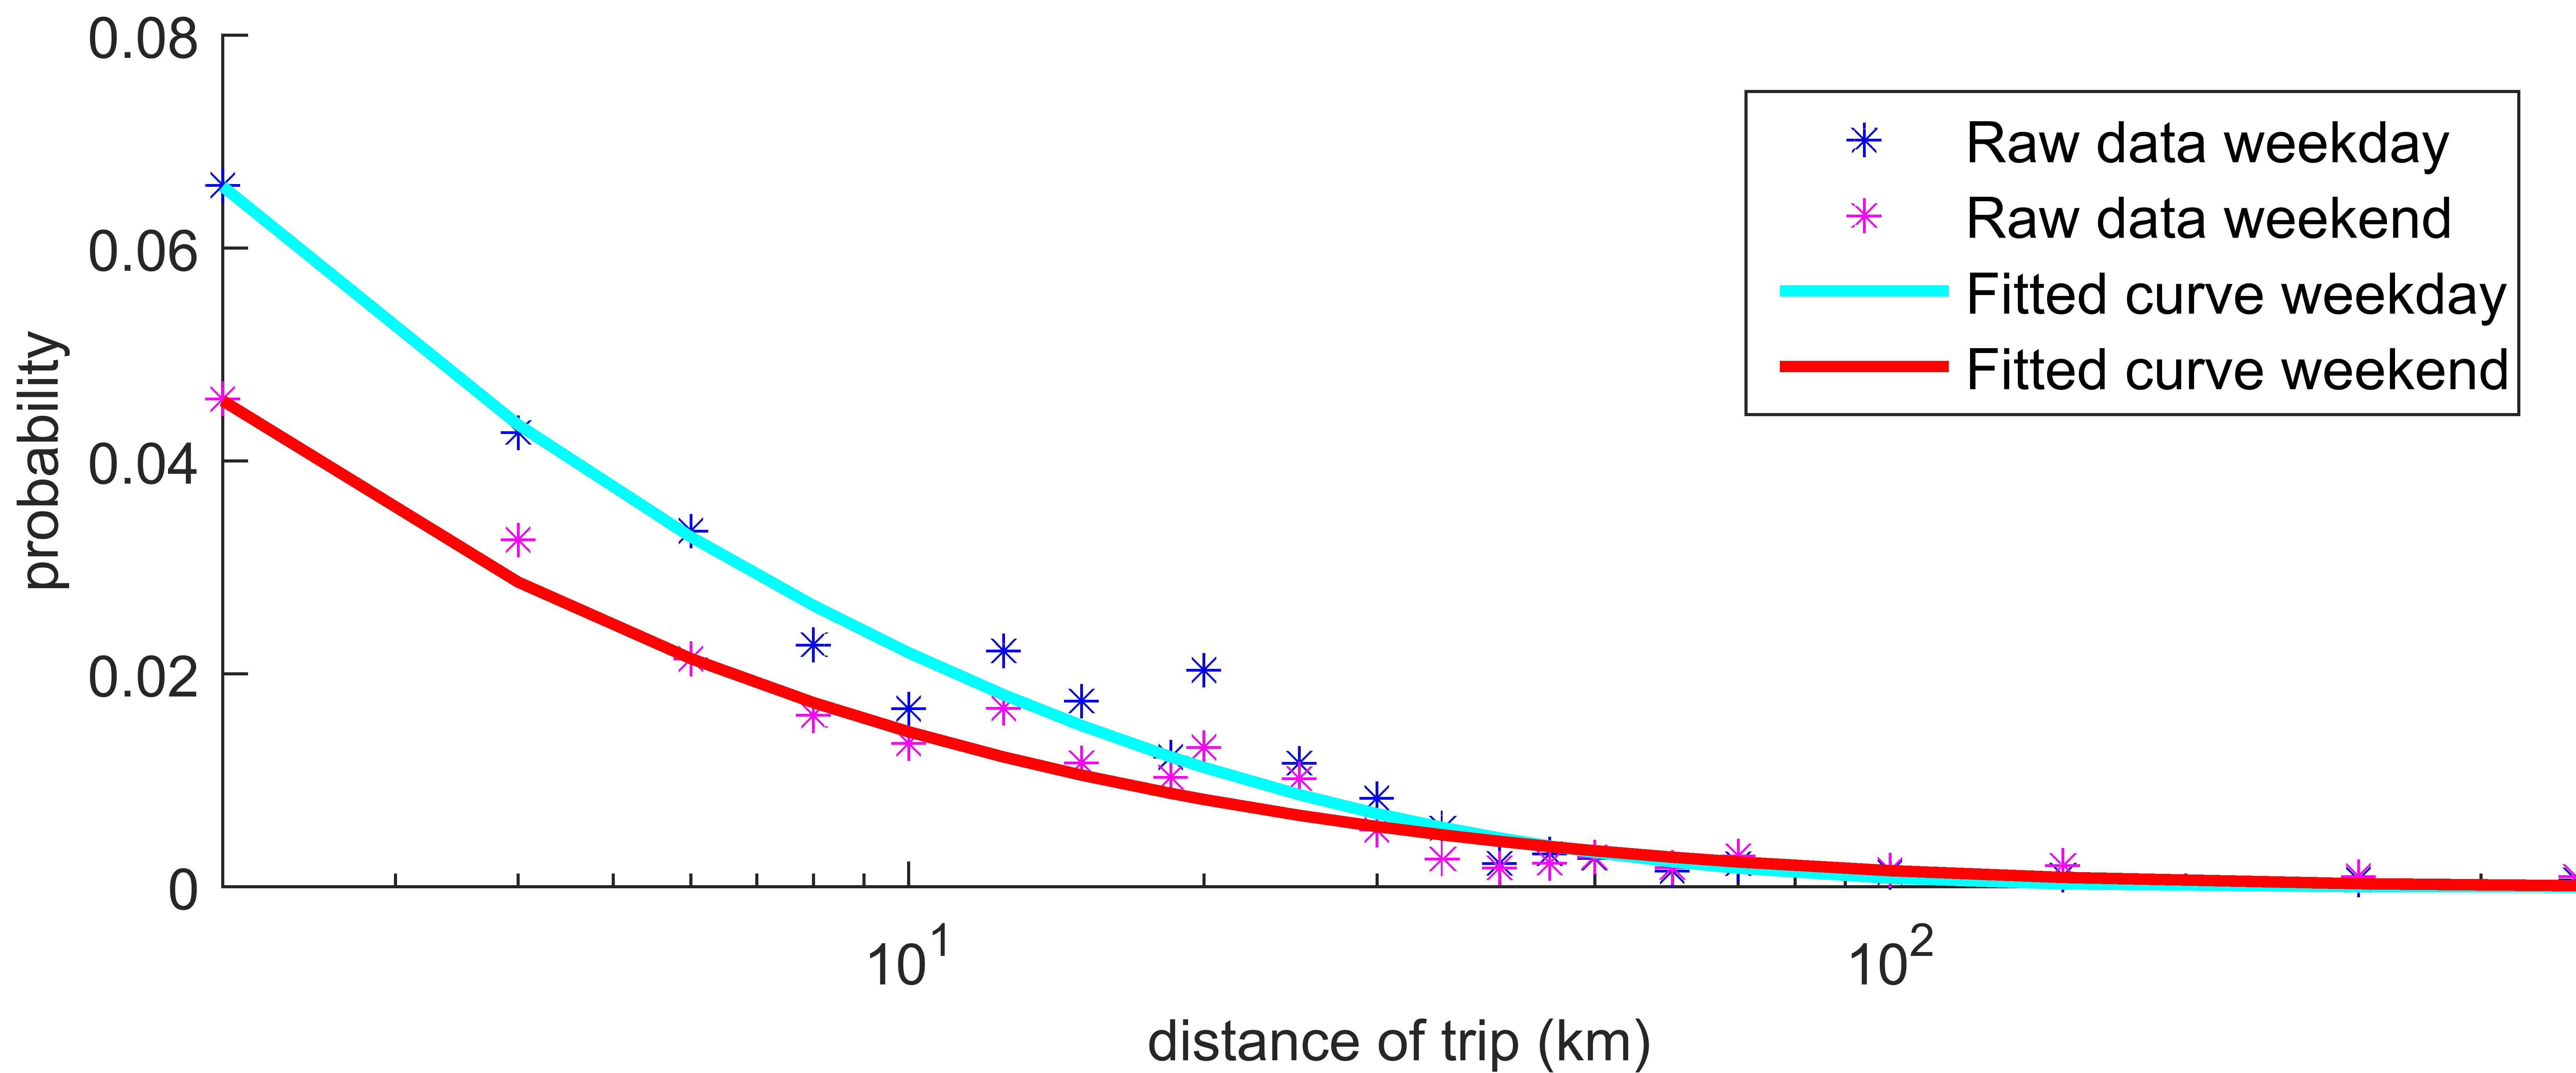
\includegraphics[width=0.8\textwidth]{_chapter4/fig/trip-distance-probability}
	\caption{The probability of a trip being of a particular distance during a weekday, extrapolated into a Weibull distribution (RMS error: $3.791\%$).}
	\label{ch4:fig:trip-distance-probability}
\end{figure}

 
In addition to these probabilities, an average driving speed of 56 kmh (35 mph) and an average driving energy efficiency of 0.1305 kWh/kmh (0.21 kWh/mph) are taken from \cite{UKGovernmentDigitalService2013}.
Using the predicted driving distance and average driving speed with the driving energy efficiency, it is possible to estimate an EV's energy demand upon arrival.
Starting to charge from this arrival time until the energy demand has been met allows the generation of an estimated charging profile of a single EV.
To do this, a maximum charging power of the U.K.'s average household circuit rating (i.e., 7.4 kW) and an immediate disconnection of the EV upon charge completion were assumed \cite{EVHomeCharging}.

Generating several of those charging profiles and aggregating them produces an estimated charging demand for an entire fleet of EVs.
To provide an example, charge demand profiles for 50 EVs were generated, aggregated and plotted in Figure~\ref{ch4:fig:aggregated-ev-power}.
This plot shows the expected magnitude and variability in energy demand that is required to charge several EVs at consumers' homes based on the vehicles' daily usage.

This model's EV charging behaviour has been implemented to reflect EV demand if applied today without widespread smart charging infrastructure. It does therefore reflect the worst case scenario. Future smart-charging schemes would mitigate the currently present collective EV charging spike, yet the implementation and validation of available smart-charging schemes lies beyond the scope of this paper. This model's data were used to feed additional demand into the power network models, which are outlined in the next section.

\begin{figure}\centering
 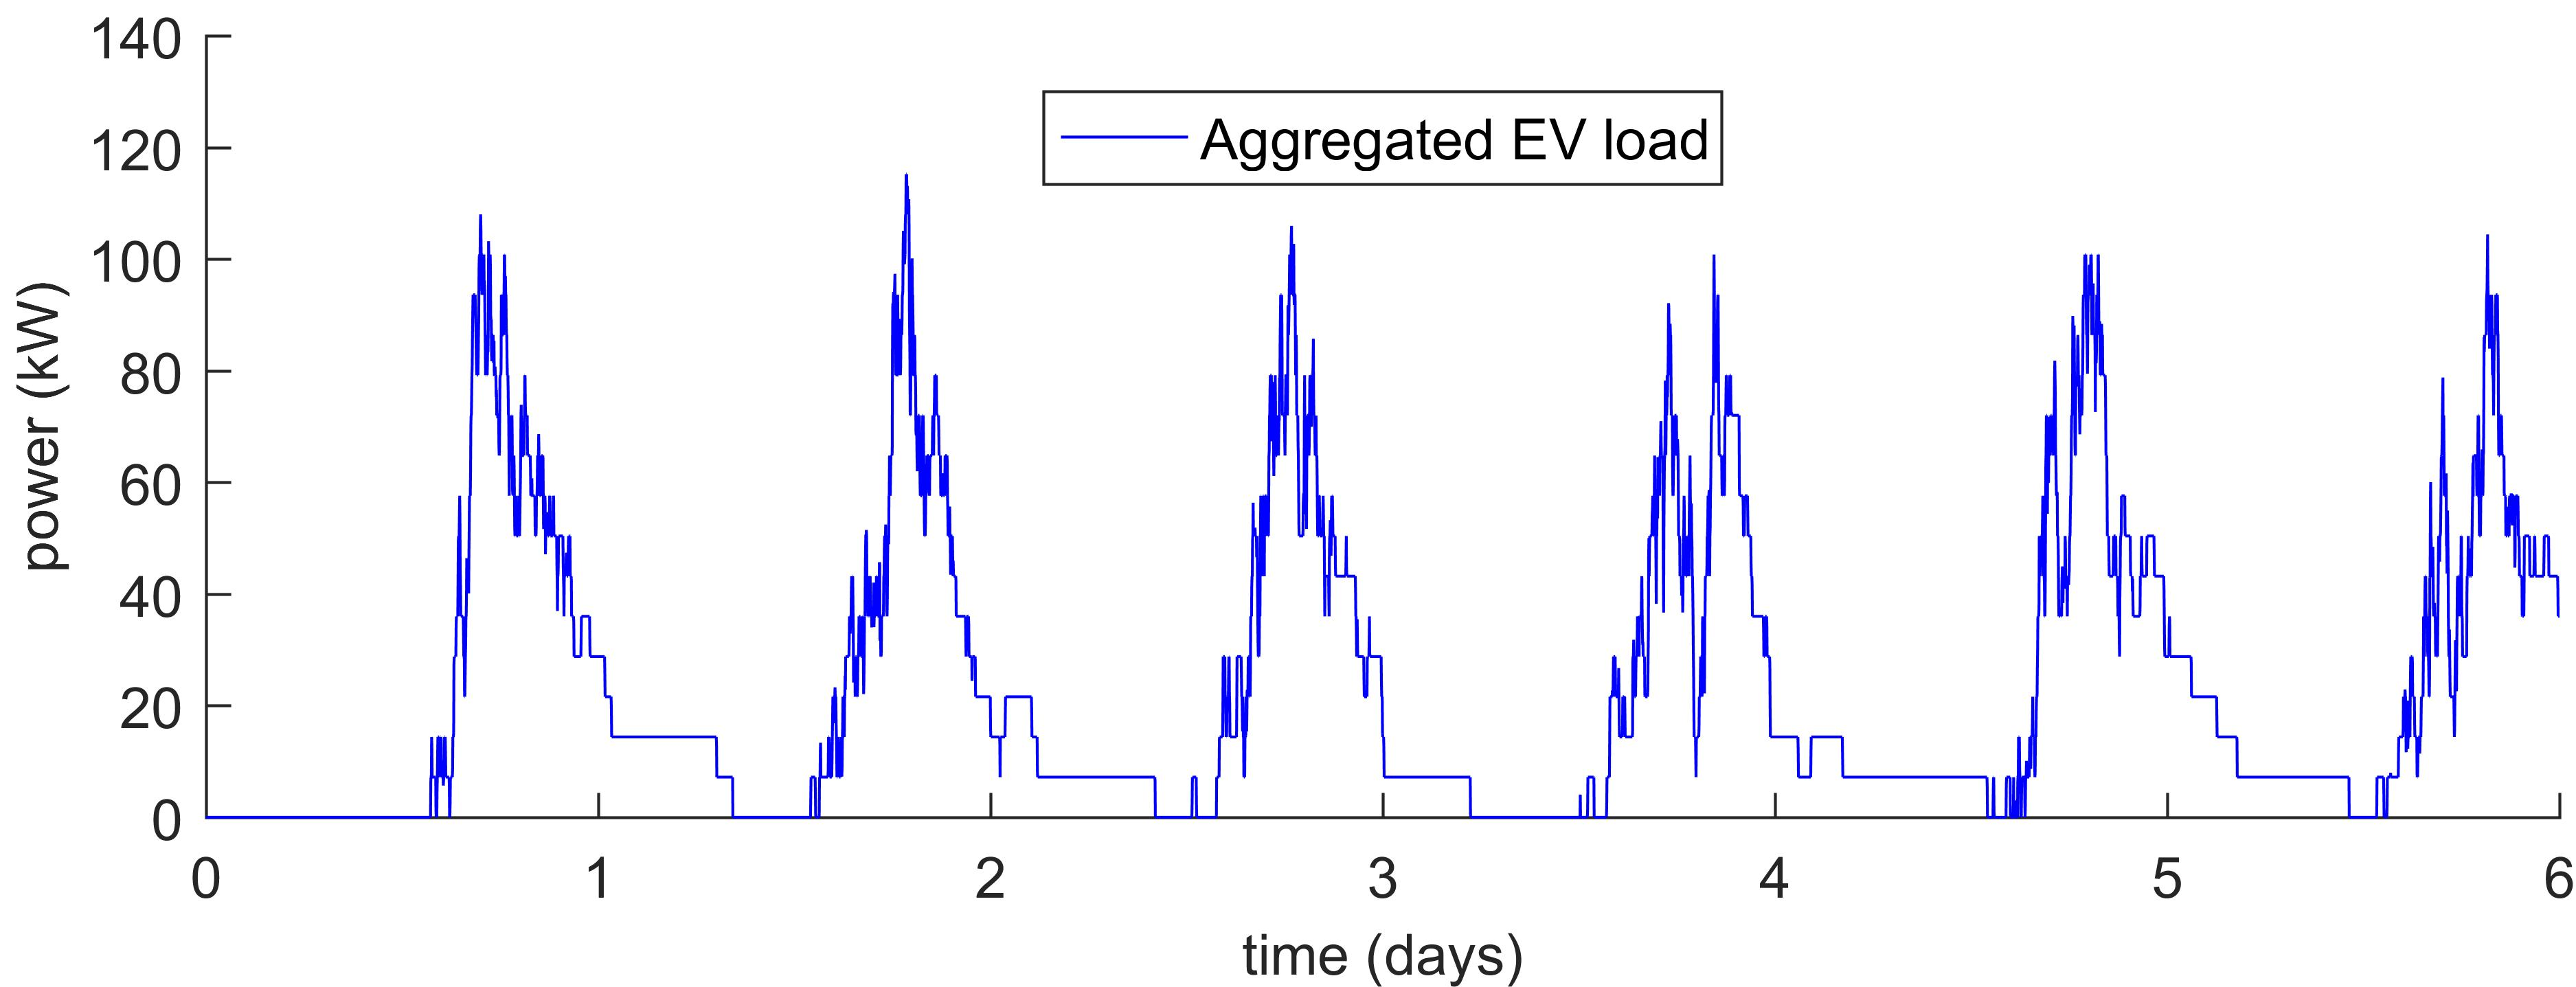
\includegraphics[width=0.8\textwidth]{_chapter4/fig/aggregated-ev-power}
 \caption{Excerpt from the aggregated 50 EVs; charging powers that were each generated from the empirical models.}
 \label{ch4:fig:aggregated-ev-power}
\end{figure}


\subsection{Battery Modelling}

In this chapter the same BESS model is used, that has already been introduced in Chapter~\ref{ch1} of this thesis (i.e. see Section~\ref{ch1:subsec:battery-model}).
Nonetheless, in the following paragraphs, this model's details are reminded, since this battery model consists of a self-discharge loss, $\mu$, that is dependent on the current State Of Charge (SOC) and an energy conversion efficiency, $\eta$, to compute the amount of energy that is lost when charging or discharging this battery. 
%This model has also been was used in \cite{Rowe2013, Rowe2014, Rowe2014a, Zangs2016},

\nomenclature[L]{$p_\text{bat}(t)$}{Battery power at time $t$, where $p_\text{bat}(t) \in \mathbb{R}$}
\nomenclature[L]{$\text{SOC}(t)$}{Battery state of charge at time $t$}
\nomenclature[L]{$\Delta\text{SOC}(t)$}{Change in SOC during time period $\Delta t$}
\nomenclature[L]{$\mu$}{Self-discharge loss factor}
\nomenclature[L]{$\eta$}{Energy conversion efficiency}
\nomenclature[L]{$\text{SOC}_\text{min}$}{Minimum rated SOC for limited battery operation}
\nomenclature[L]{$\text{SOC}_\text{max}$}{Maximum rated SOC for limited battery operation}
\nomenclature[L]{$C$}{Battery capacity}
\nomenclature[L]{$P_\text{max}$}{Power rating of battery}
\nomenclature[L]{$\Delta t$}{Sampling period}

When an ideal battery charges or discharges, the change in SOC is related by the battery power, $p_\text{bat}(t)$.
When sampling battery operation at a regular period, $\Delta t$, then the energy transferred into the battery can be described as $p_\text{bat}(t)\Delta t$.
The change in SOC for this ideal battery, $\Delta SOC$, is therefore defined as:

\begin{equation}
\Delta \text{SOC}(t) := \frac{p_\text{bat}(t)\Delta t}{C} = \text{SOC}(t) - \text{SOC}(t-\Delta t)
\label{ch4:equ:change-soc}
\end{equation}


The self-discharge loss is included in this ideal battery model to represent the continual loss of energy in the battery typical of chemical energy storage.
This loss, $\Delta\text{SOC}_\text{self-discharge}$, is defined to be proportional to the current SOC and is determined using the self-discharge loss factor, $\mu$:

\begin{equation}
	\Delta\text{SOC}_\text{self-discharge}(t) := \mu\text{SOC}(t)
	\label{ch4:equ:self-discharge-loss}
\end{equation}


Additionally, to represent the losses in the power electronics and energy conversion process, an energy conversion loss, $\Delta\text{SOC}_\text{conversion}(t)$, is defined.
This loss is proportional to the rate at which the battery's SOC changes, by using the energy conversion efficiency, $\hat{\eta}$ as follows:

\begin{equation}
	\Delta\text{SOC}_\text{conversion}(t) := \hat{\eta}\Delta\text{SOC}(t) \text{ where } \hat{\eta} \in (0, 1]
	\label{ch4:equ:conversion-loss}
\end{equation}


Here, the conversion losses in the power electronics are reflected as an asymmetric efficiency, which depends on the direction of the flow of energy.
This is done by charging the battery at a lower power when consuming energy and discharging it more quickly when releasing energy.
Mathematically, this can be represented as:

\begin{equation}
\hat{\eta} =
	\begin{cases}
		\eta &\text{if } \Delta\text{SOC}(t) \geq 0 \\
		\frac{1}{\eta} &\text{if } \Delta\text{SOC}(t) < 0
	\end{cases}
\label{ch4:equ:energy-conversion-adjustment}
\end{equation}


When substituting the self-discharge loss from Equation~\ref{ch4:equ:self-discharge-loss}, $\Delta\text{SOC}_\text{self-discharge}$, and conversion losses from Equation~\ref{ch4:equ:conversion-loss}, $\Delta\text{SOC}_\text{conversion}$, into the SOC evolution equation, the full battery model, i.e. the transition from $\text{SOC}(t)$ to $\text{SOC}(t+\Delta t)$, can be summarised as follows:

\begin{equation}
	\begin{split}
		\text{SOC}(t+\Delta t) :&= \Delta\text{SOC}(t) - \Delta\text{SOC}_\text{self-discharge}(t) - \Delta\text{SOC}_\text{conversion}(t)\\
		&= (1-\mu)\Delta\text{SOC}(t) - \hat{\eta}\Delta\text{SOC}(t)	
	\end{split}
	\label{ch4:equ:soc-transition}
\end{equation}


In addition, both the SOC and the battery power, $p_\text{bat}(t)$, are constrained due to the device's maximum and minimum energy storage capabilities, respectively $\text{SOC}_\text{max}$ and $\text{SOC}_\text{min}$, and maximum charge and discharge rate, $P_\text{max}$.
These limitations are captured in Equations~\ref{ch4:equ:soc-range} and Equation~\ref{ch4:equ:charge-discharge-range}, respectively.

\begin{equation}
\text{SOC}_\text{min} \leq \text{SOC}(t) \leq \text{SOC}_\text{max}
\label{ch4:equ:soc-range}
\end{equation}


\begin{equation}
\left|p_\text{bat}(t)(t)\right| \leq \text{P}_\text{max}
\label{ch4:equ:charge-discharge-range}
\end{equation}


\subsection{Network Models}
\label{ch4:subsec:network-models}

Similar to Chapter~\ref{ch1} of this thesis, the Open Distribution System Simulator (OpenDSS), developed by the Electronic Power Research Institute (EPRI), was used in order to simulate the LV energy distribution networks.
It requires element-based network models, including line, load and transformer information, and generates realistic power flow results.

\begin{figure}\centering
	\subfloat[]{%
		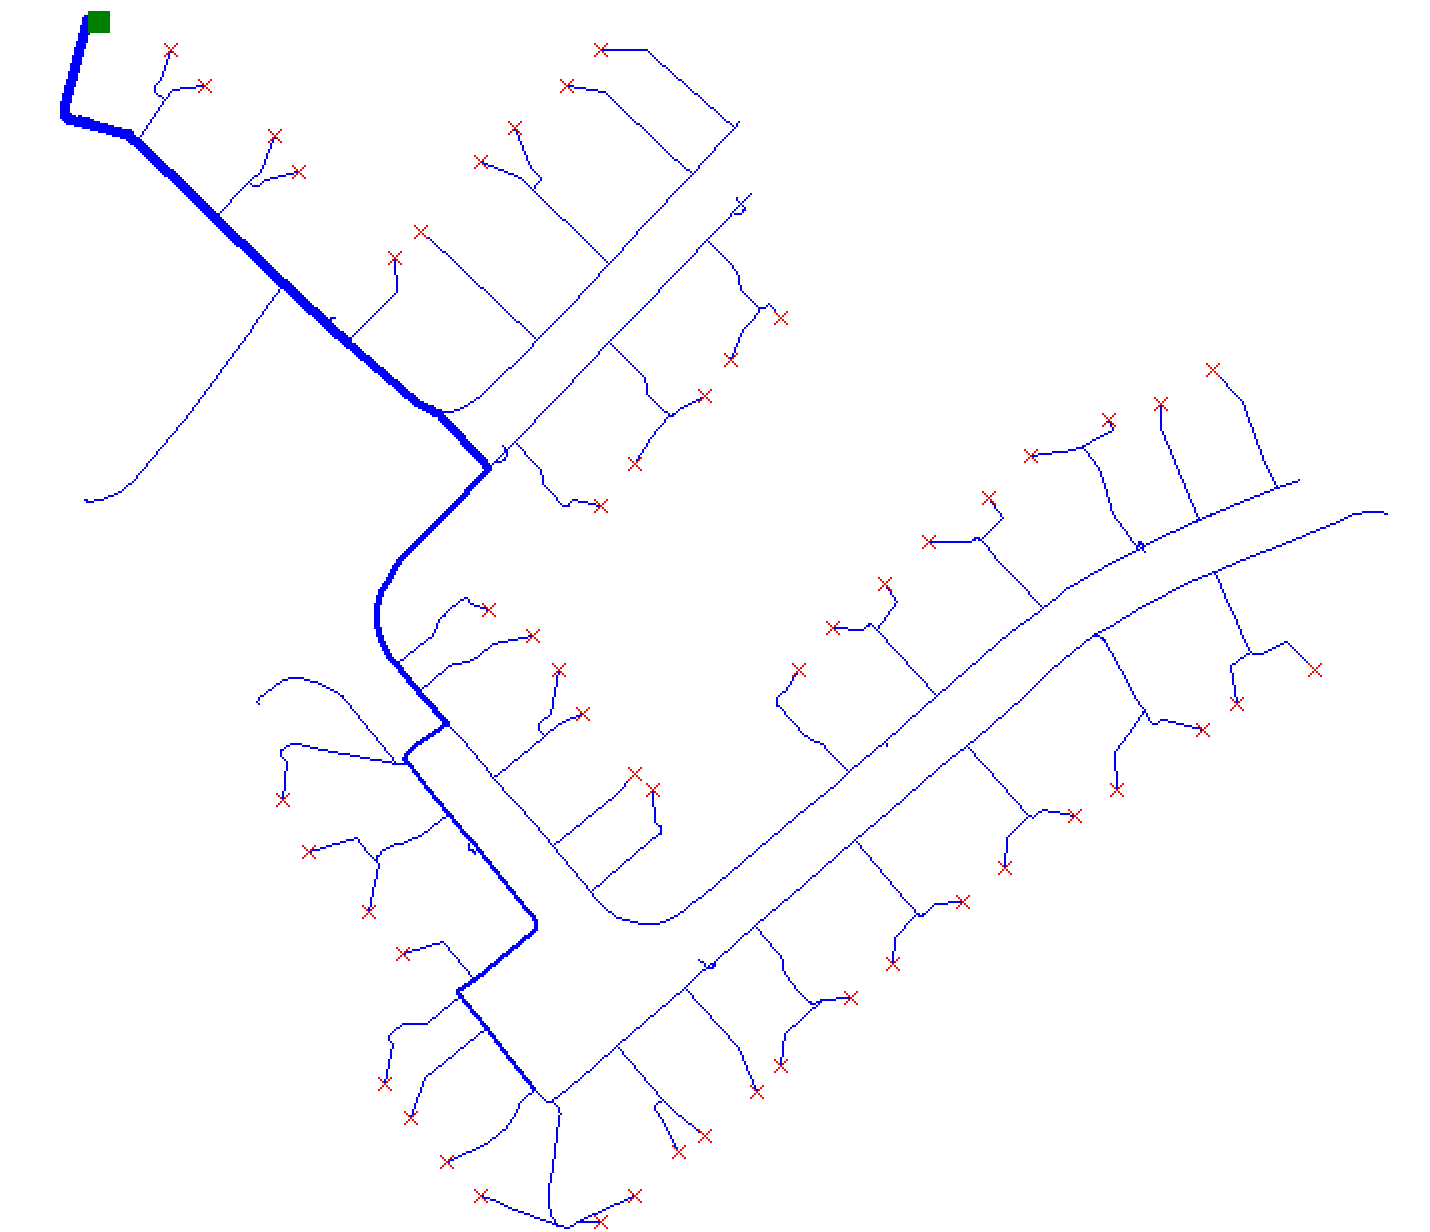
\includegraphics[width=0.5\linewidth]{_chapter4/fig/network-EULVFeeder}%
		\label{ch4:subfig:network-ieee}%
	}
	\subfloat[]{%
		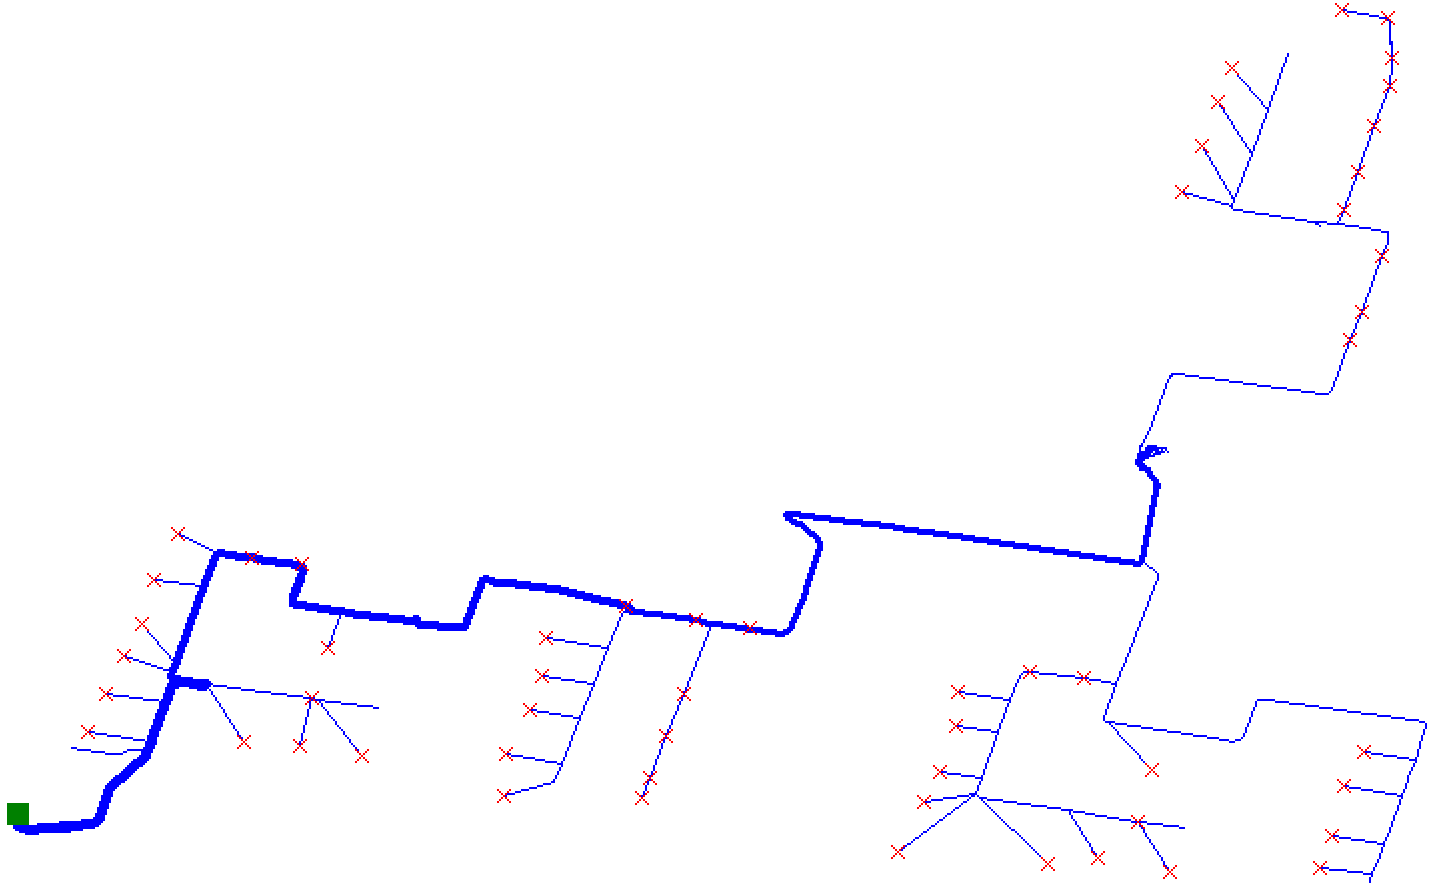
\includegraphics[width=0.5\linewidth]{_chapter4/fig/network-Deepdale_FD01}%
		\label{ch4:subfig:network-ssen}%
	}
	\caption{Sample OpenDSS power networks, where consumers are indicated as red crosses and 11/0.416-kV substations are marked with a green square. Here, (a) is the IEEE PES EU LV test feeder, and (b) is a SSEN Common Information Model (CIM) based feeder}
	\label{ch4:fig:network}
\end{figure}


Simulations were conducted using the IEEE's European Low Voltage Test Feeder \cite{EULVFeeder2015} and six detailed U.K. feeder models, that are based on real power distribution networks and provided by Scottish and Southern Electricity Networks (SSEN).
The SSEN circuit models were provided as Common Information Models (CIM) during the collaboration on the New Thames Valley Vision Project Project (NTVV) \cite{NTVV2016}.
An example of the IEEE EU LV Test feeder and a UK feeder provided by SSE-PDEN are shown in Figure~\ref{ch4:subfig:network-ssen} and Figure~\ref{ch4:subfig:network-ssen}, respectively.
A summary of these model's parameters is given in the Table~\ref{ch4:tab:model-parameters}.

\begin{table}\centering
\begin{tabular}{r | c | c c c c c c}
%\multirow{2}{*}{\textbf{Parameter}} & \textbf{IEEE EU} & \multicolumn{6}{c}{\multirow{2}{*}{\textbf{SSEN LV Feeders}}}\\
% & \textbf{LV Test Feeder} & \\
Parameter & IEEE Feeder & \multicolumn{6}{c}{SSEN Feeders}\\
\hline
network No. & 1 & 2 & 3 & 4 & 5 & 6 & 7\\
\hline
no. of customers & 55 & 56 & 53 & 91 & 59 & 88 & 37\\
mean customer load (VA) & 227 & 227 & 231 & 241 & 224 & 237 & 237\\
max. customer load (kVA)& 16.8 & 16.8 & 16.8 & 19.5 & 16.8 & 19.5 & 16.8\\
mean net. load (kVA)& 24.4 & 24.9 & 23.9 & 41.9 & 25.6 & 38.9 & 16.3\\
max. net. load (kVA)& 72.6 & 72.7 & 72.2 & 92.9 & 73.5 & 89.6 & 60.5\\ 
%\hline
%Customer connection & Single-phase & \multicolumn{6}{c}{Single-phase}\\
%\hline
%\multirow{2}{*}{Feeder line model} & Three-phase & \multicolumn{6}{c}{Three-phase}\\
% & implicit-neutral & \multicolumn{6}{c}{explicit-neutral}\\
\end{tabular}
\caption{Network model parameters.}
\label{ch4:tab:model-parameters}
\begin{tabular}{ccc}
%\multicolumn{1}{c}{\footnotesize $^1$ These networks are shown in Figure~\ref{ch4:fig:network}.}
\end{tabular}
\end{table}


Throughout the remainder of this chapter, all excerpt and time series results were extracted from experiments with the IEEE EU LV Test feeder (i.e., Network No. 1).
Any further results are then based on an aggregation of all networks to include their network diversity in the analysis.

The same model-derived EV data and IEEE EU LV Test feeder consumer demand profiles were used for all simulations.
The resulting demand profiles therefore represent the total daily electricity demand of households with connected EVs.
These profiles were sampled at $\Delta t = 1\text{ min}$.
The OpenDSS simulation environment was controlled using MATLAB, achieved through OpenDSS's Common Object Model (COM) interface and accessible using Microsoft's ActiveX server bridge.


